\section{Execution and deployment.}\label{sec:network}
In section \ref{sec:vlbi} we presented the two operational mode we are
targeting for the software correlator: \emph{batch-execution} and
\emph{real-time}. Grids have a long history in running batch jobs and
grid-middleware is now doing a good job on this task. Therefore
running a software correlator without real-time requirements is
feasible on most grids. However for real-time applications the
situation is much more complex, as the grid infrastructure and
corresponding middleware have to provide guarantees on the Quality of
the Service that match the application's requirement. As these issues
are still evolving rapidly we are testing these aspects of \scarie\ on
an experimental grid called DAS-3 and its associated network service
called StarPlane.

\subsection{Real-time and quality of service}
The term \emph{real-time} has many definitions in the computer science
community, in this paper we will consider that a \emph{real-time}
computation is a computation in which: \emph{the amount of buffering
  for an infinitely long experiment will only require a finite amount
  of buffers}. This is a formal way to define a process in which the
incoming data are "consumed" by the computation as fast as they are
generated. This definition also imply that once the application is
started the allocated "space" on the resources will be maintained
during the complete execution.

The major resources \scarie\ is using are: the networking bandwidth, 
the computation resource and the disk-space if the data have 
to be saved. The sharing of the computational resource is now
a well understood process. Most of the time it is part of the 
execution service, this service taking a description of the 
application deployment as well as a description of the 
requested service (and resource). The execution service 
allocating rights to access the requested services or 
resource and, finally, if all part of the request 
are fulfilled, deploy the application. 
\begin{figure}
  \centering
  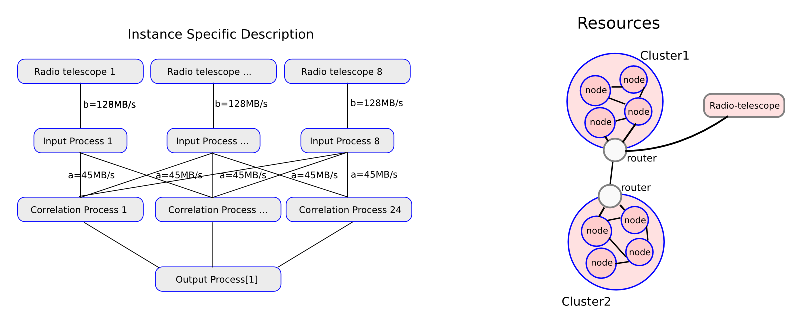
\includegraphics[width=\textwidth]
    {img/mapping.eps}
    \caption{Left: An specific instaInce of an experiment. Right: The
      resource set. Resource allocation and application scheduling
      have to map the left side to the resources. }
  \label{fig:mapping}
\end{figure}
\marginpar{NGHK: Can the figure go?}
The simplest way to offer guaranteed service over a shared resource
can be done restricting the access to only one user at a time. This
approach is used in the DAS-3 grid (based on SGE) in which a node
allocated is simply unusable by other users. Same principle could be
applied to the complete grid including its networks and other
resources. A more complicated, but really interesting approach consist
of sharing the resource under the arbitration of a third party that
will insure that each application is using only the allocated part of
the resource. This is the approach that is often refereed in
bibliography as Layer-2/3 QoS for network services, or the recently
added Completely Fair Scheduler (per application control on their cpu
usage) or IO- (per application IO-bandwith arbitration). In a very
general point of view all these technologies permit to virtualize the
resource thus permit to build on top of a real grid a complete virtual
environment based on user requirements.

\subsection{Running \scarie on \das3 and Starplane}
Networking issues are one of the challenges of the \scarie\ project.
The regular Internet best-effort Layer3 IP routing has great
flexibility but is slow and unpredictable; on the other hand,
dedicated \textit{lightpaths} as available in \textit{lambda
  Grids}~\cite{eslea-2007}, with their predictable delays and
throughputs offer good performances and guarantee on the Quality of
Service (QoS). This is the approach that is used in \scarie\ to
delivered the data from the radio-telescope to the computation center.
Giving end user an access to dedicated connection has been implemented
in many of the current research and education networks. The Dutch
National Resarch and Education network SURFnet is one of them.
SURFnet6 deploys multiple fiber optic rings that connect the academic
and research locations around The Netherlands.

For the correlation process we are experimenting on the \das3\ grid.
The \das3\ supercomputer~\cite{das3} was deployed in the summer of
2007. It is composed of fives clusters located in the Netherlands and
connected by a photonic network called StarPlane. The StarPlane
project manages eight wavelengths in one of the SURFnet6 optical
rings.  The goal of the project is to build a network service that
permits \textit{application-controlled photonic network and
  node-to-node traffic isolation}. The novelty of the StarPlane
project lies in its attempt to build a virtual network service at the
lowest possible networking layer: the photonic layer for the optical
part and ethernet-layer2 for the connexion to the nodes. This has the
advantage to improve performances and to dramatically reduce the cost
(the price or the energy) per byte transfered \cite{}\marginpar{TODO}.

StarPlane manages eight wavelengths in one of the SURFnet6 optical
rings. The goal of StarPlane is to build an
\textit{application-controlled photonic network}. The novelty of the
StarPlane project lies in its attempt to build a virtual network
service at the lowest possible networking layer. This has the
advantage to improve performances and to dramatically reduce the cost
(the price or the energy) per byte transfered \cite{}\marginpar{TODO}.
A complete virtual network for an application can then be build using
only vlan-on-mac layer 2 switches and layer-1 photonic lighpath. The
other novelty is that the photonic lightpath can dynamically be
reorganized to adapt to the user-application requests.  \marginpar{DM:
  layer 0 for the optical part and layer 2 for the LAN connexion to
  the nodes}

\subsection{Benchmarks on DAS-3}
\scarie~ and StarPlane have parallel roadmaps. Hence the complete
approach cannot be tested yet. We have conducted correlator
performances test using \das3. The current software correlator is
currently able to perform a 4x128Mbps experiment at 20\% of the
real-time speed using a total of 16 (quad core 2.0Ghz cpu) nodes.

In parallel with the benchmarks of the correlator, we are also testing
the capabilities of StarPlane to do high performance traffic isolation
that is needed for real-time correlation. As the computing power of
one cluster may not be sufficient, it might be necessary to distribute
the workload over several locations. Therefore high-bandwidth, QoS
aware, network connections are needed between the clusters. At the
time of writing StarPlane has implemented the service that allows a
program to build and allocate a lighpath between two clusters on
demand. We tested this feature by running two client-server
applications transmitting data between clusters.

The network traffic of the two applications is depicted in
Figure~\ref{fig:timing}.  At the start of the application, a request
for lighpath allocation is issued (arrow 1). After a while the
throughput drops because the second application starts sending data as
well (arrow 2).  As long as the lighpath is not ready (photonic
switching takes 10 minutes) the application is sending the traffic to
the default 1Gb/s ethernet route; when the lighpath is ready (arrow 3)
the traffic is rerouted to the lightpath.

\begin{figure}[ht]
  \centering
  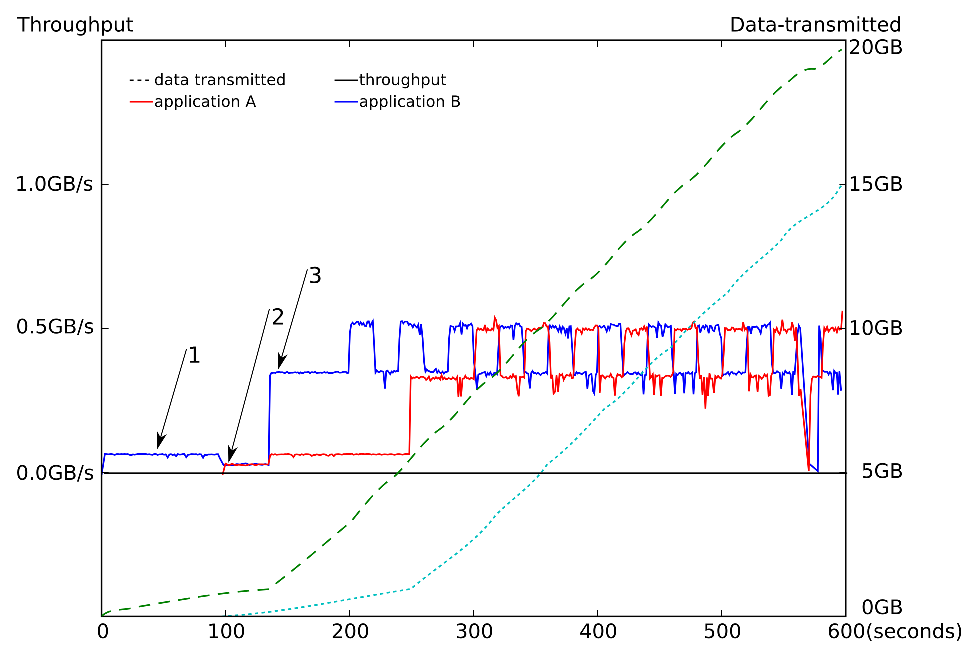
\includegraphics[width=\textwidth] {img/timing.eps}
  \caption{\label{fig:timing} Two application are started at time
    (arrow 1) and (arrow 2). The two applications have to share the
    1Gbps network bandwith. When a lighpath is allocated (arrow 3) the
    increase in performance is clearly visible.}
\end{figure} 

The results of this experiment rise questions, as the secured
lightpath is supposed to deliver reliably "550MB/s" of throughput
between a pair of cluster. In Figure~\ref{fig:timing} we can see a
periodic artifact, the traffic falling down to 300MB/s for few
seconds. A second issue to investigate is that from time to time the
lighpath connectivity disapears entirely (e.g. at second 580). We are
currently working with Starplane team to understand and solve these
problems.


%%% Local Variables:
%%% mode: latex
%%% TeX-master: "Ingrid"
%%% End:
